\documentclass{article}

\author{John McAvoy}
\date{}

\usepackage{amsmath}
\usepackage{amsfonts}
\usepackage{graphicx}
\usepackage{url}
\usepackage{mcode}
\usepackage{amsmath}
\usepackage{color}
\usepackage{xfrac}
\usepackage{flushend}
\usepackage{wrapfig}
\usepackage{float}
\usepackage{color}   %May be necessary if you want to color links
\usepackage{hyperref}
\hypersetup{
    colorlinks=true, %set true if you want colored links
    linktoc=all,     %set to all if you want both sections and subsections linked
    linkcolor=blue,  %choose some color if you want links to stand out
}
\usepackage [english]{babel}
\usepackage [autostyle, english = american]{csquotes}
\MakeOuterQuote{"}

\usepackage[margin=1in]{geometry}
\usepackage{float}

\title{ABET Internal Network Documentation}

\begin{document}

\maketitle

\tableofcontents

\section{Setting Up Internal Network}
The internal ABET network is comprised of two routers: a WiFi station that connects to "Rowan\_IOT" WiFi and hosts a DCHP server that routes the internet connection through its
ethernet ports, and a wireless access point (AP) that connects to the WiFi station via ethernet and hosts its own DHCP server and broadcasts a WiFi signal called "ABET WiFi."
All clients are connected to the AP router, two ABET desktops and two printers are connected via ethernet and all other devices connect via the WiFi by connecting to "ABET
WiFi" (Figure \ref{fig:network}).

\begin{figure}[H]
  \centering
  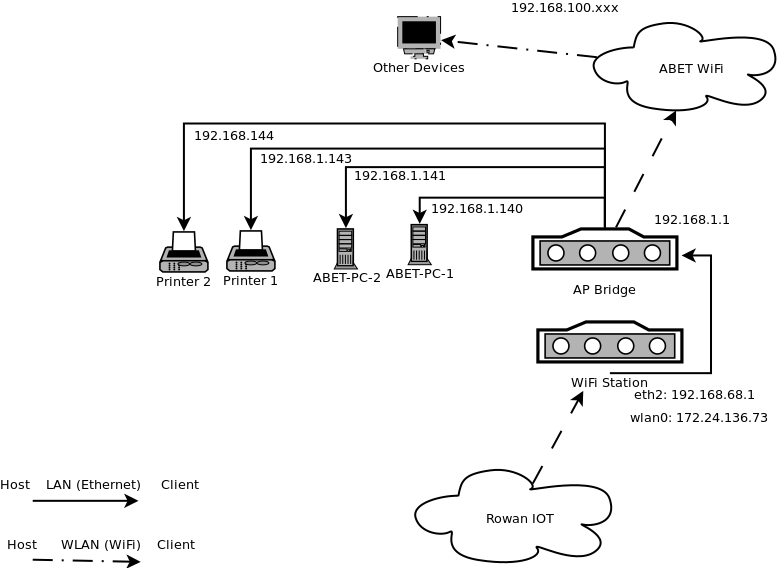
\includegraphics[scale=0.30]{./img/network.png}
  \caption{ABET Network Diagram}
  \label{fig:network}
\end{figure}

\subsection{Rowan\_IoT WiFi Station}
A MikroTik router was used as the WiFi station. The router is configured in
"router" mode, wireless set to automatically acquire an IP address from
Rowan\_IOT, and set configure its local network with the router's local IP address as
192.168.88.1 (this is it's IP relative to other devices connected to the router)
a netmask of 255.255.255.0, and a DHCP range of 192.168.88.10-192.168.88.255
(this is the range of IP addresses that the router assigns to devices that
connect it) (Figure \ref{fig:01_quick_set}).


\begin{figure}[H]
  \begin{center}
    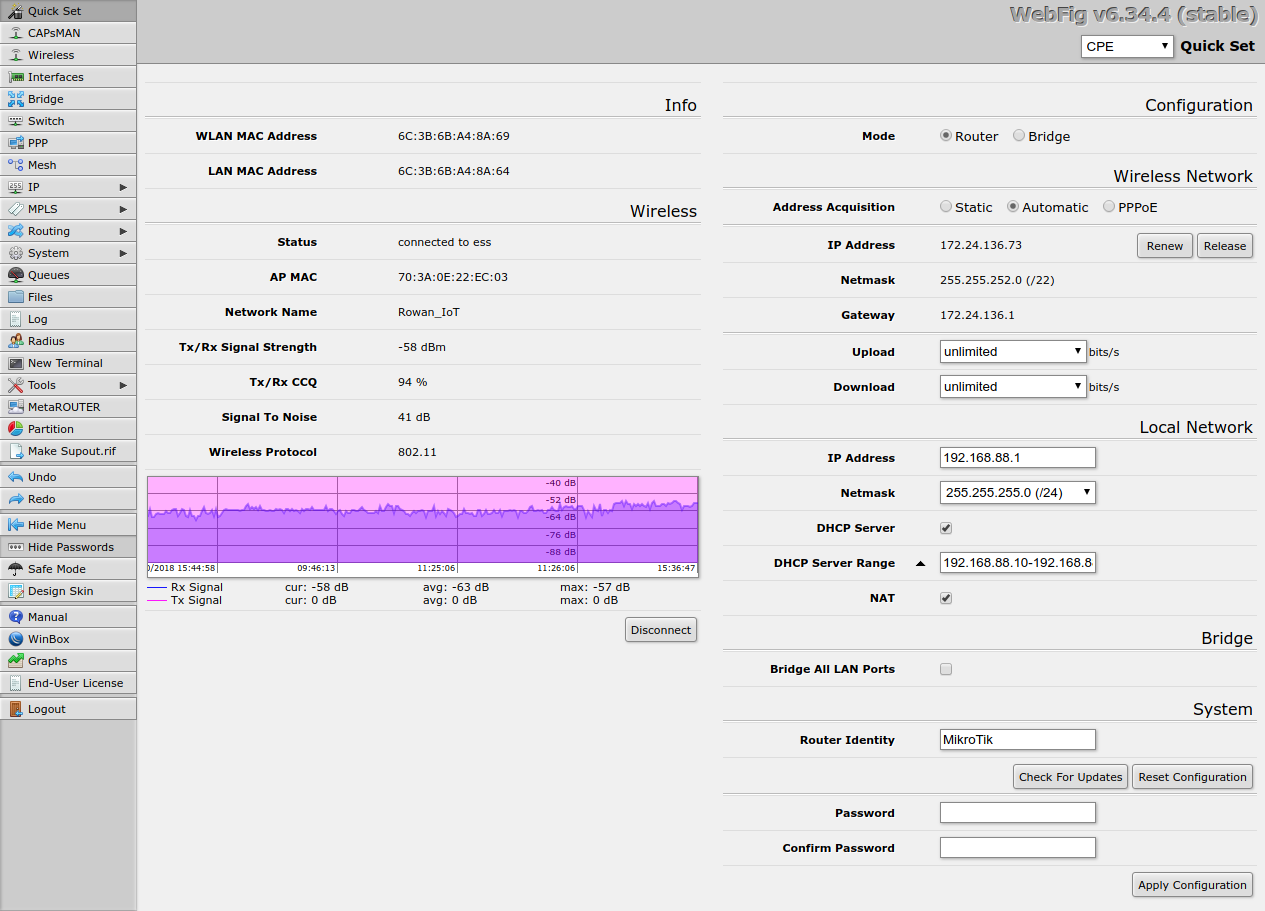
\includegraphics[scale=0.30]{./img/mikrotik/01_quick_set.png}
  \end{center}
  \caption{MikroTik Setup: Quick Set}
  \label{fig:01_quick_set}
\end{figure}

The wireless interface of this router was called "wlan1" and it was configured
to connect to Rowan\_IOT (Figures \ref{fig:02_wireless} and
\ref{fig:03_wlan1_interface}).

\begin{figure}[H]
  \begin{center}
    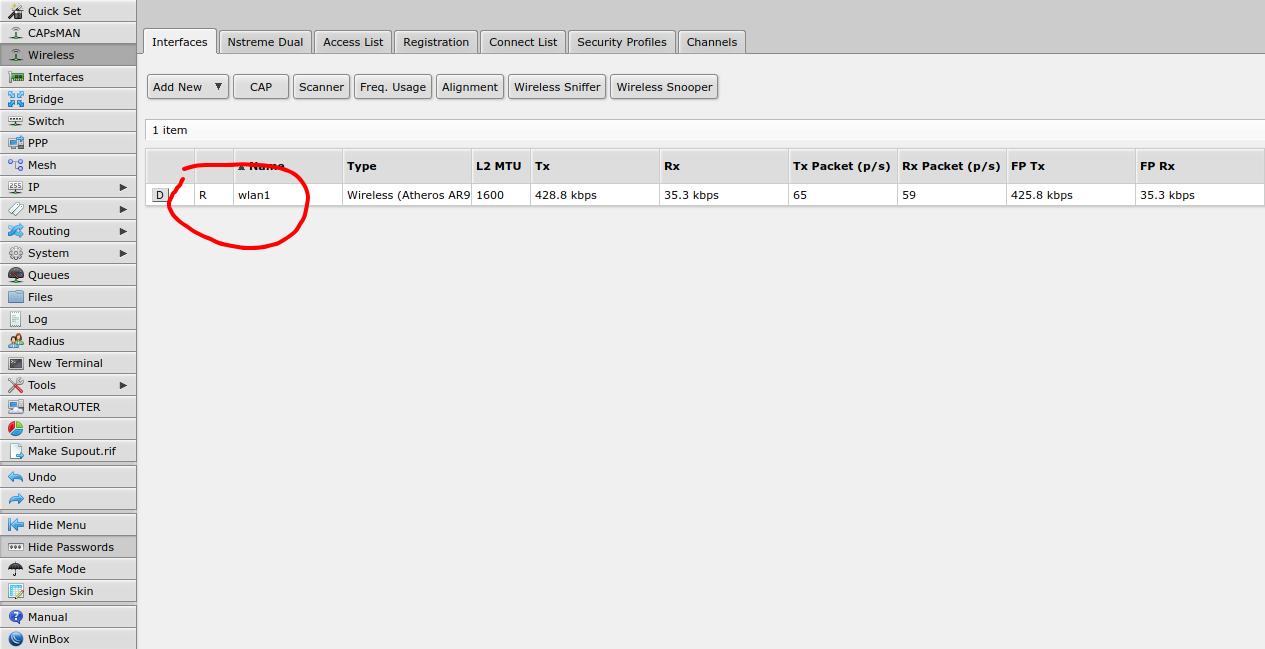
\includegraphics[scale=0.30]{./img/mikrotik/02_wireless.png}
  \end{center}
  \caption{MikroTik Setup: Wireless Configuration}
  \label{fig:02_wireless}
\end{figure}

\begin{figure}[H]
  \begin{center}
    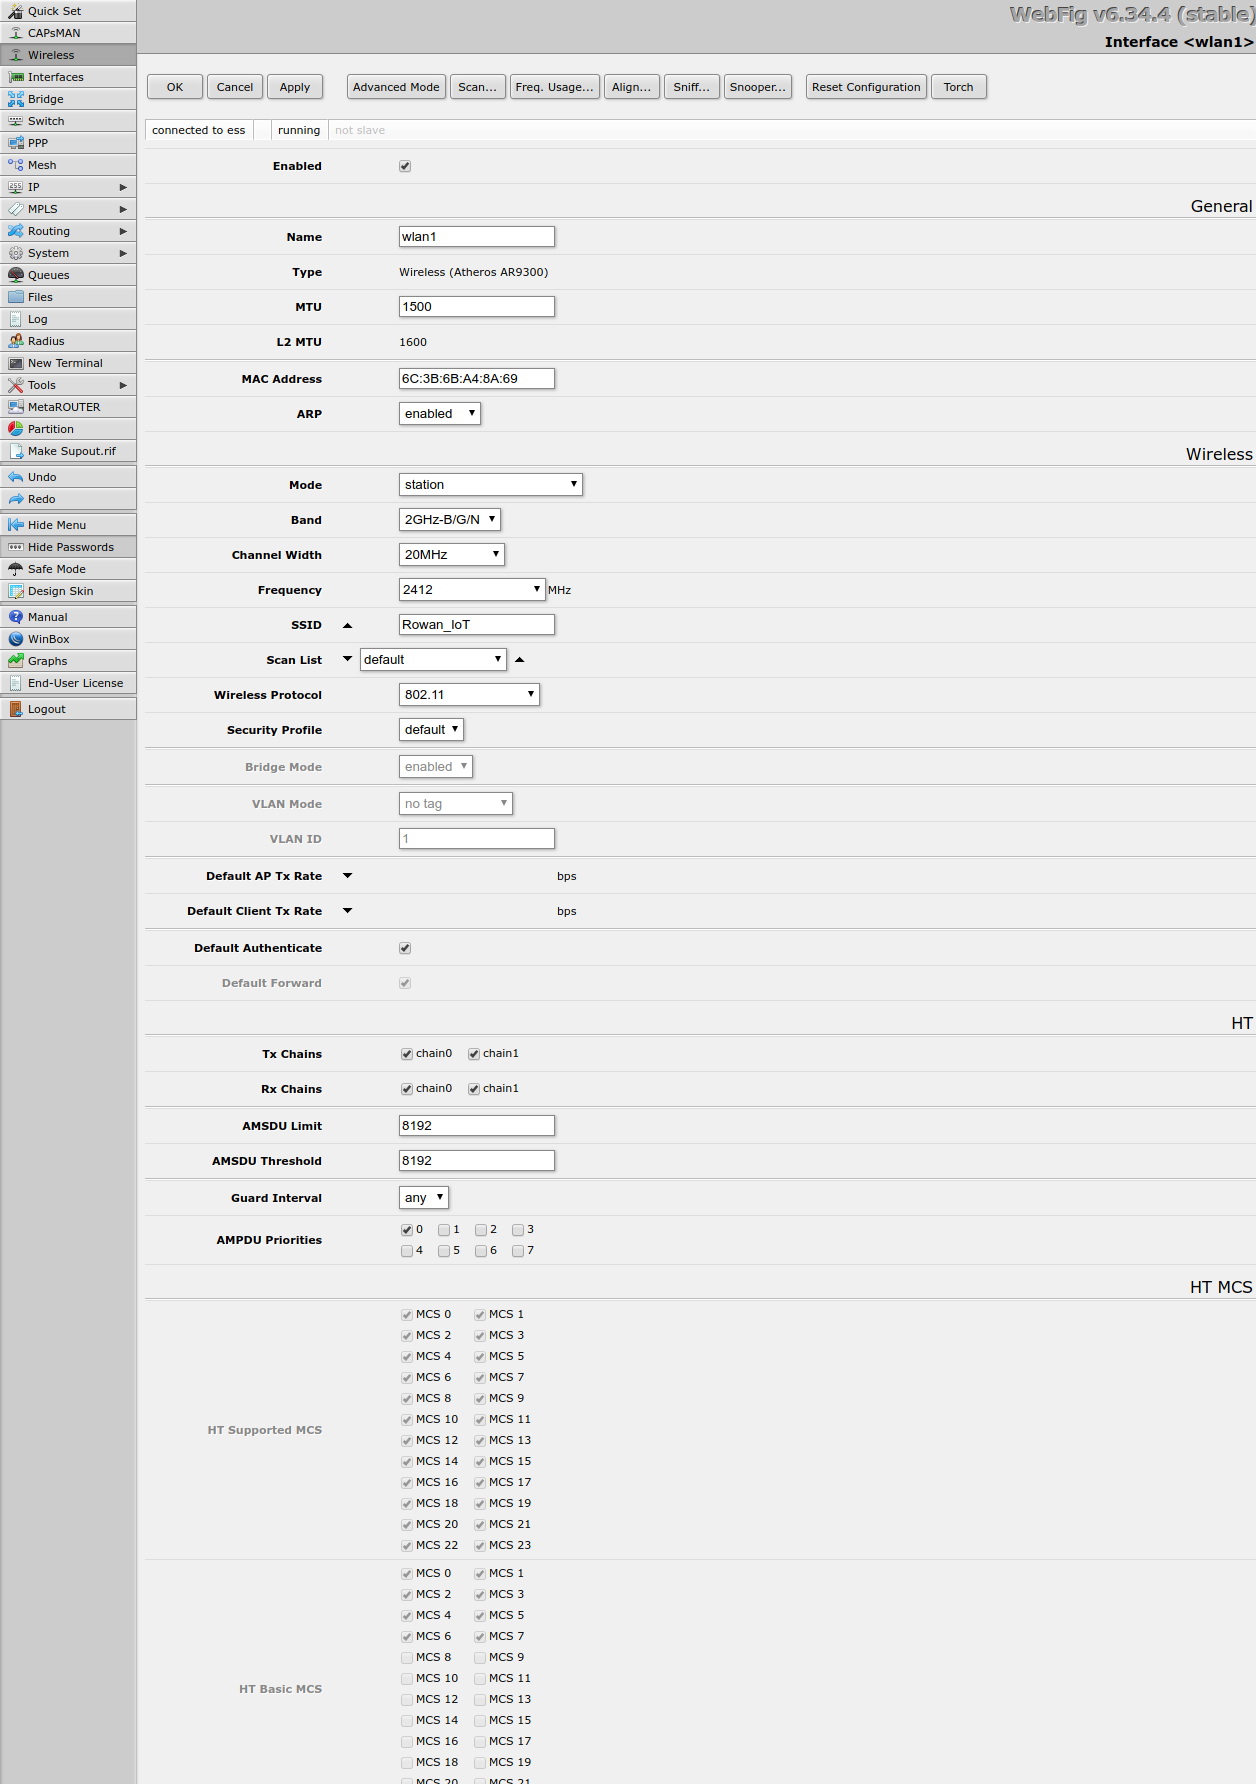
\includegraphics[scale=1]{./img/mikrotik/03_wlan1_interface.png}
  \end{center}
  \caption{MikroTik Setup: wlan1 Interface Configuration}
  \label{fig:03_wlan1_interface}
\end{figure}

The router has five ethernet interfaces (eth1-eth5) and a bridge that connects
the interfaces together (Figure \ref{fig:04_interfaces}).

\begin{figure}[H]
  \begin{center}
    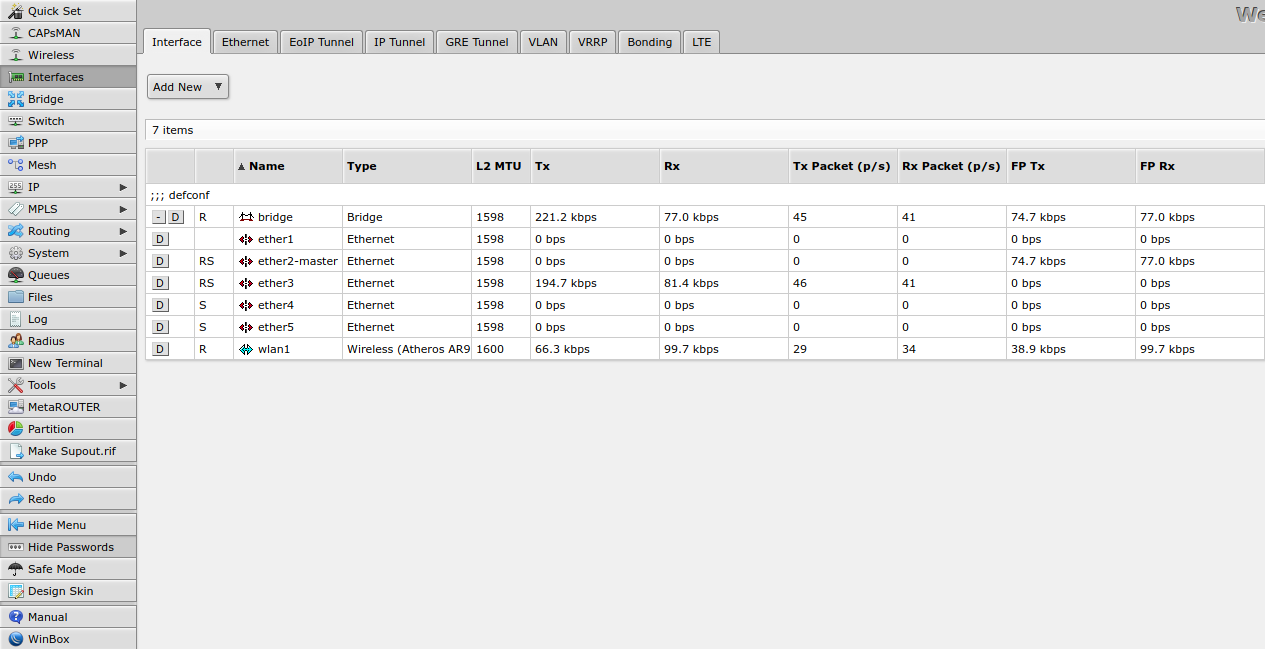
\includegraphics[scale=0.30]{./img/mikrotik/04_interfaces.png}
  \end{center}
  \caption{MikroTik Setup: Interfaces Overview}
  \label{fig:04_interfaces}
\end{figure}

The purpose of this router is to transfer the wireless Rowan\_IOT connection to an ethernet
connection. In order to do this, we need to set the router up as a DHCP client
so it can connect to Rowan\_IOT similar to a computer, so we need to configure
the DHCP client to use the wlan1 interface (Figures \ref{fig:05_dhcp_client} and
\ref{fig:06_dhcp_wlan1}).

\begin{figure}[H]
  \begin{center}
    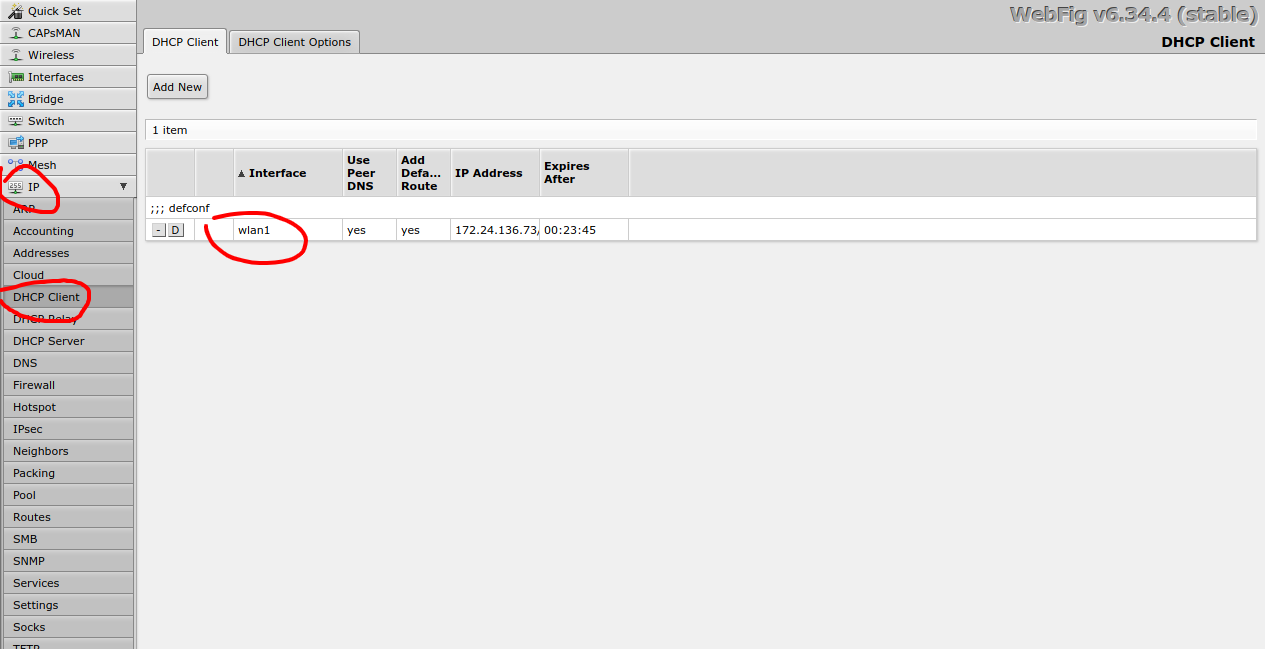
\includegraphics[scale=0.30]{./img/mikrotik/05_dhcp_client.png}
  \end{center}
  \caption{MikroTik Setup: DHCP Cliet Configuration}
  \label{fig:05_dhcp_client}
\end{figure}

\begin{figure}[H]
  \begin{center}
    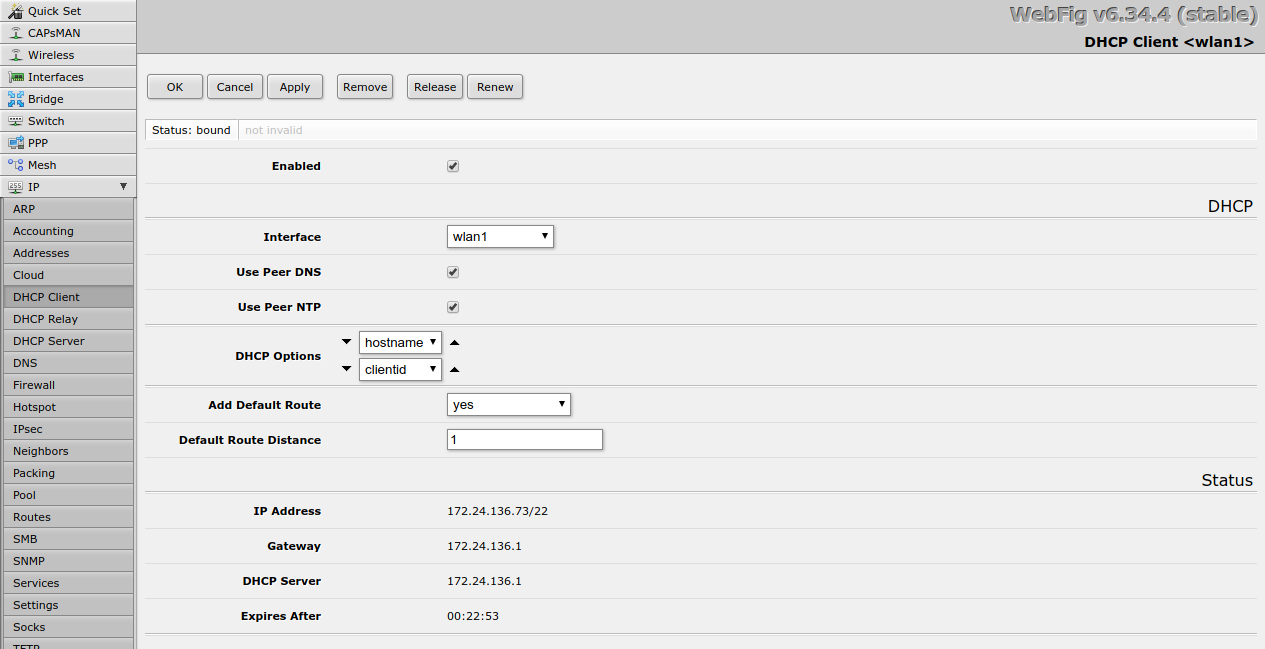
\includegraphics[scale=0.30]{./img/mikrotik/06_dhcp_wlan1.png}
  \end{center}
  \caption{MikroTik Setup: DHCP wlan1 Configuration}
  \label{fig:06_dhcp_wlan1}
\end{figure}

\subsection{WiFi Station to AP Bridge}
A Linksys Router with a custom DD-WRT firmware was used as the AP bridge (Access
Point Bridge). This configuration sets the router as a wireless access point
that takes an ethernet connection and bridges the connection to its other 4
ports as well as hosts a wireless network that is also bridged to the ethernet
connection. This allows us to host our own ABET\_WiFi using the connection from
the MikroTik router (Figures \ref{fig:01_basic_setup} and
\ref{fig:02_ap_bridge}).

\begin{figure}[H]
  \begin{center}
    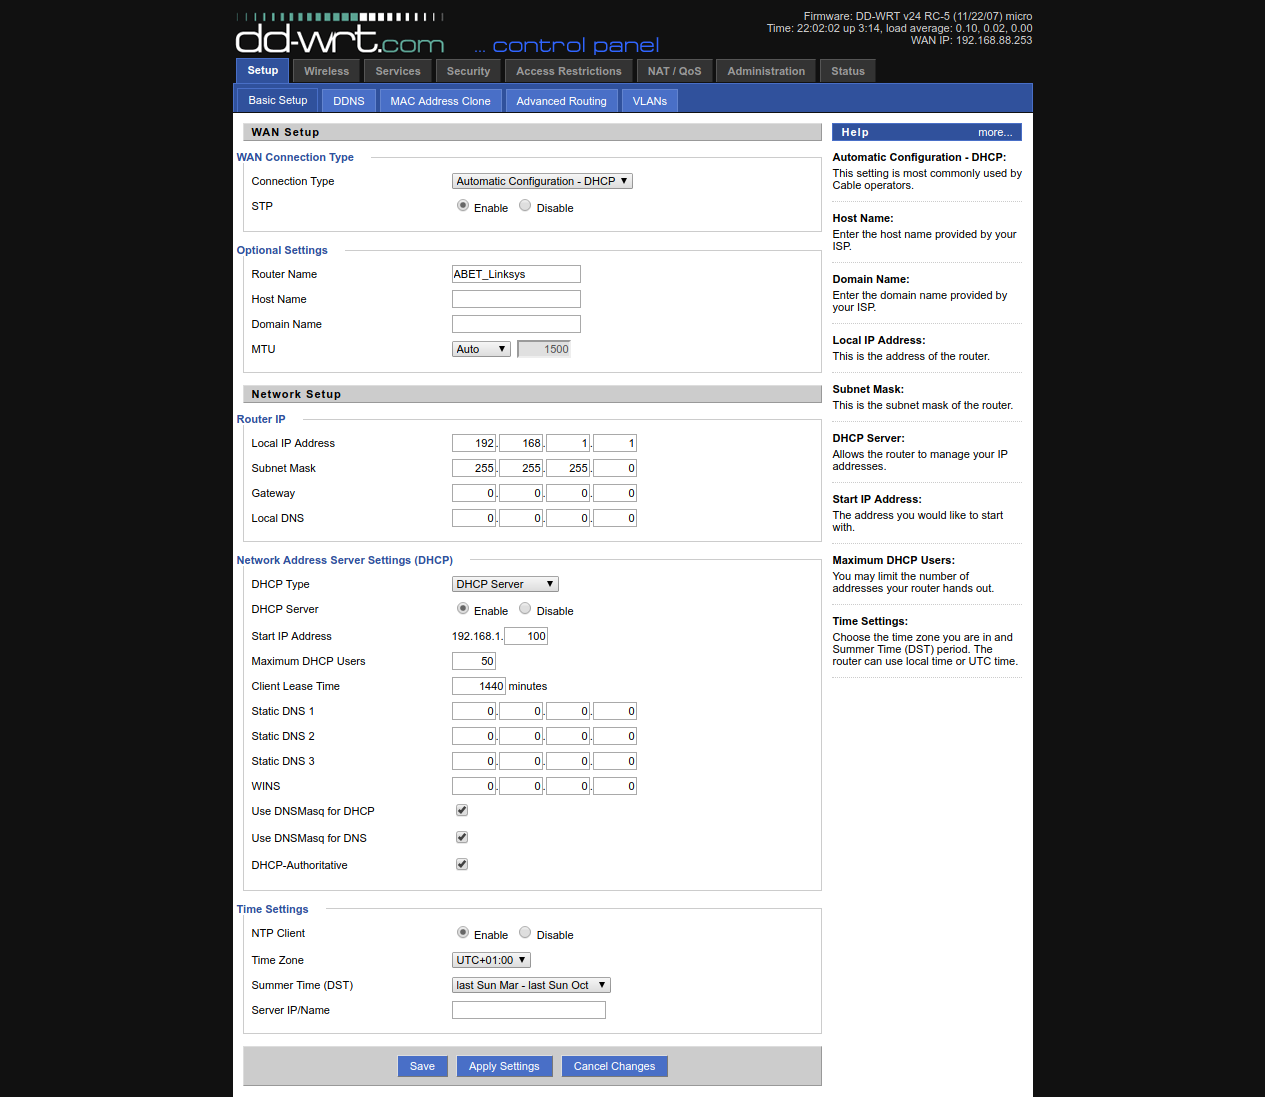
\includegraphics[scale=0.30]{./img/ddwrt/01_basic_setup.png}
  \end{center}
  \caption{DDWRT Setup: Basic Setup}
  \label{fig:01_basic_setup}
\end{figure}

\begin{figure}[H]
  \begin{center}
    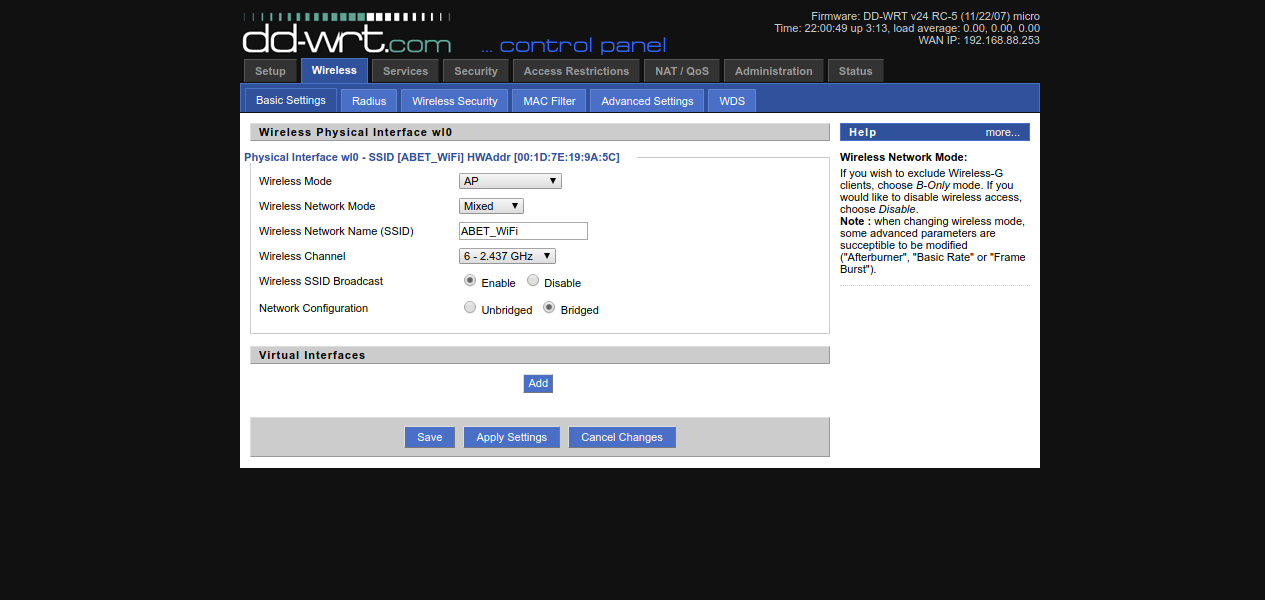
\includegraphics[scale=0.30]{./img/ddwrt/02_ap_bridge.png}
  \end{center}
  \caption{DDWRT Setup: AP Bridge Mode}
  \label{fig:02_ap_bridge}
\end{figure}

The next step is setting up a DNS which points \url{http://abetshare} to the
ABET\_1 IP address (Figure \ref{fig:03_dns}).

\begin{figure}[H]
  \begin{center}
    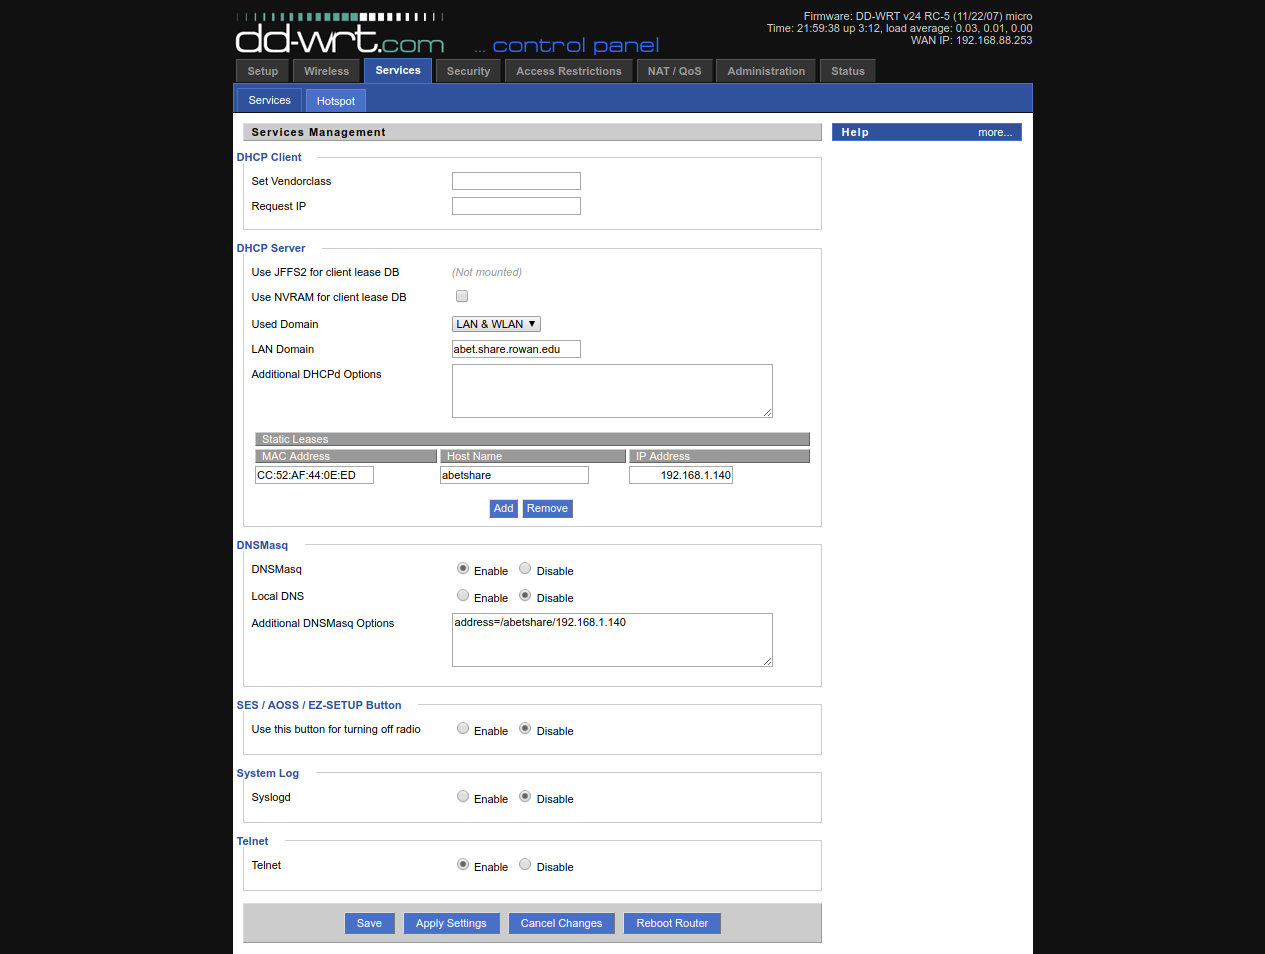
\includegraphics[scale=0.30]{./img/ddwrt/03_dns.png}
  \end{center}
  \caption{DDWRT Setup: DNS}
  \label{fig:03_dns}
\end{figure}

\section{Setting Up the Printers}
Two printers were shared on the ABET network. This was done by
connecting each printer to the WiFi to AP Bridge via Ethernet. One printer was
connected via USB to ABET\_1 and the other to ABET\_2 and the printer drivers were
installed on each desktop.

\section{Setting Up the Desktops}
The two ABET desktops, ABET-PC-1 and ABET-PC-2, are public desktops that are connected to the ABET network. One of the desktops hosts the ABET fileshare while the other
continuously syncs with the fileshare.

\subsection{Convert a "Rowan Desktop" to an "ABET Desktop"}
Both desktops were taken from the labs in REXT, which means they are configured to connect to Rowan's Network and only Rowan Administrators can modify networking and install
software on them. In order to get these desktops to do what we want for the ABET network, we need to "un-Rowanify" them, meaning get them to boot to a fresh install of
Windows where we have control over how they are configured.

\subsubsection{Add a New Internal Drive}
The first step in converting the desktops is to open them up, replace the current bootable drive that boots the locked-down Windows with a new drive on which we will install a
fresh version of Windows. The following steps will accomplish this:

\textit{Note: When taking apart desktops, you should \textbf{never} force anything open, remove rivets, or
        need to use any power tools. If you are ever unsure how to detach a component, refer to the manufacturer's documentation.}
\begin{enumerate}
    \item{Opening the Desktop Chassis}\\
        The procedure to remove the side panel varies based on the manufacturer of the case, however it should be intuitive, it typically involves unscrewing two large screws
        on the back of the case or squeezing a tab that unhooks the side panel. Just make sure you have a clean working environment so things don't get lost. Once the side
        panel is removed, you may find that the inside of the desktop is dusty, in which case you'll want to use compressed air to clean out the dust.

    \item{Locating the Drive Bay}\\
        The drive bay is a compartment that holds the hard drives (HDD's) or solid state drives (SSD's) which are hold the system's internal storage. The drive bay is usually
        in the front-bottom corner of the case. You should see two cables that go to a drive in the drive bay, one from the motherboard, and one from the power supply, this drive is the one you will be
        replacing.

    \item{Replacing the Bootable Drive}\\
        Similar to opening the side panel, there should be an intuitive way to open the drive bay and remove the bootable drive. Remove the cables from the drive, unmount the
        drive from the drive bay, label this drive and store it in a safe place (you will have to re-install this drive when it goes back to being a Rowan desktop so don't
        lose it), place a new HDD of SSD into the drive bay, and connect the two cables you disconnected to the new drive. At this point, you should be able to install an OS
        on this drive.

        %\textit{There is a chance that you live in the significant future, in which case there may not be a drive bay or any 2.5-inch drives. In which case there is a small
        %    M.2 SSD on the motherboard that is the bootable drive that you will need to replace.}

\end{enumerate}

\subsubsection{Fresh Install Windows}

\begin{enumerate}
  \item{Insert a bootable Windows install media into the desktop.}\\

  \item{Entering the BIOS or UEFI}\\
    Before you turn on the computer, it is important that you know how to
    configure the booting sequence to boot from you bootable Windows drive instead of
    the empty drive that you inserted earlier. To do this, you will need to
    enter the BIOS (Basic Input/Output System) or the UEFI (Unified Extensible
    Firmware Interface). This is is done by pressing a specific key on the
    keyboard during booting. Usually this key is one of the function keys
    F1-F12, the Delete Key, or the Escape Key. You can try to mash all the keys
    randomly at first and see if a text-based menu opened up, or you can look at
    the manufacturer's specific instructions for entering the BIOS.

  \item{Modifying the Boot Order}\\
    In the BIOS/UEFI menu, you should see a menu that says "Boot Order" or
    something similar. Navigate to that menu and you should see be able to
    modify the boot sequence that the computer performs at startup. The highest
    item in the boot order is the drive that the computer tries to boot from if
    it can. If that drive is unavailable, it goes to the next drive in the list
    and tries to boot from it. Modify this order so that the first drive in the
    list is your Windows USB flash drive or CD. Once this is done, save and exit
    the BIOS, the computer will restart and if successful, boot into the Windows
    installation menu.

  \item{Installing Windows}\\
    The installation process for Windows should be straight-forward. Choose the
    unallocated drive to be where Windows is installed and wait for all steps to
    complete. When prompted for a system and a user account name, enter
    something like "ABET-1-PC" and "ABET-1" to keep things simple. Once
    installation is complete, you should restart enter the BIOS again and change
    the boot order again so the Windows installation drive has the highest
    priority.

\end{enumerate}

\subsection{Setting Up File Sync}

The file sync software used was Syncthing, a free, open-source, and light-weight
application that syncs folders between computers over a local network. Syncthing
was installed on both ABET desktops and used to sync the ABET\_SHARE folder on
each desktop. Configuring Syncthing is done via a web-interface and it should be
done on one desktop at a time to avoid conflicts (Figure
\ref{fig:syncthing}).

\begin{figure}[H]
  \centering
  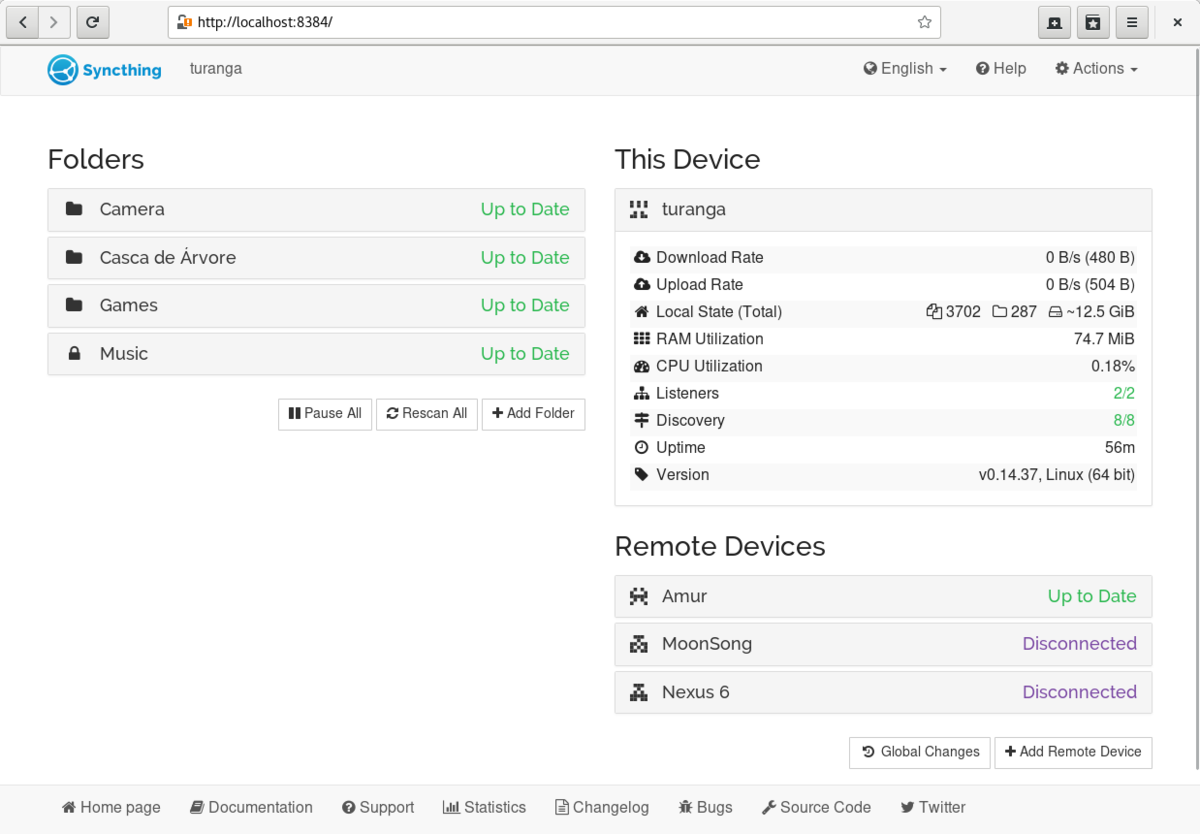
\includegraphics[scale=0.30]{./img/syncthing.png}
  \caption{Syncthing Screenshot}
  \label{fig:syncthing}
\end{figure}

\begin{enumerate}
  \item Launch Syncthing on both desktops.
  \item On ABET\_1, open the Syncthing web-interface.
  \item Select "Add Remote Device." Syncthing should be able to detect the other
    Syncthing instance it should prompt to add the other desktop in which case,
    add this device and give it a name "ABET\_2-PC". If Syncthing is unable to
    detect the other instance, you will have to manually type ABET\_2's device
    id.
  \item Next, in the main menu, select "Add Folder" and choose the ABET\_SHARE
    folder. You should see ABET\_2-PC in the sharing options menu, check the box
    next to ABET\_2-PC to share this folder with ABET\_2.
  \item Finally, on ABET\_2's Syncthing web interface, a notification will pop
    up asking to accept the ABET\_SHARE file sync. Click accept, choose its
    location as "Desktop/ABET\_SHARE."
  \item At this point, Syncthing should working on both desktops and the
    contents of the ABET\_SHARE folder should sync between both desktops.
\end{enumerate}

\subsection{Setting Up Fileshare Server}

The fileshare software used was HFS (HTTP File Share), a free, open-source, and
lightweight file server that runs on Windows. This was installed on the ABET\_1
desktop. HFS takes care of generating a web-interface for uploading and
downloading documents, all that needs to be configured is a local folder path
with the files your wish to share. A folder named ABET\_SHARE was created on the
ABET\_1 desktop and used as the entry point for the fileshare.

\begin{figure}[H]
  \centering
  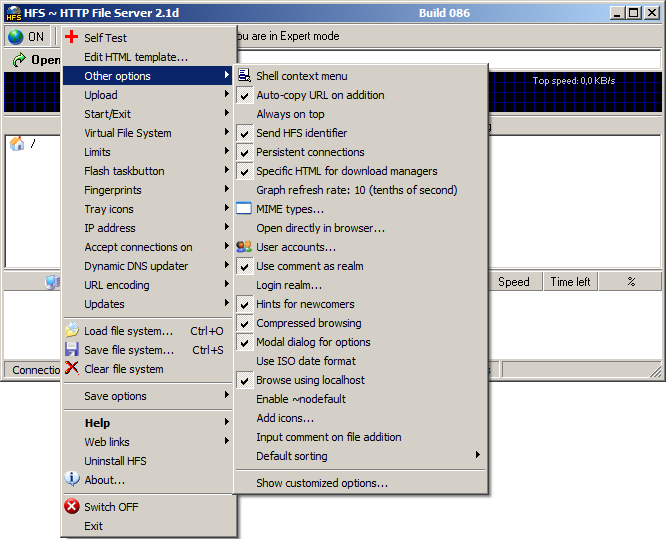
\includegraphics[scale=0.30]{./img/hfs.png}
  \caption{HFS Server Configuration}
  \label{fig:hfs}
\end{figure}

When HFS is running, you can access the fileshare webpage at the IP address of
ABET\_1 on the ABET network. To make things as seamless as possible, a DNS name
was setup on the WiFi Station to AP Bridge (Figure \ref{fig:03_dns}) so users can
type "abetshare" into their browsers instead of an IP address to access the
HFS web-interface. If configured correctly, all devices on the ABET network
should be able to access the file share as \url{http://abetshare} (Figures
\ref{fig:01_htf_home} and \ref{fig:02_hfs_abet_share}).

\begin{figure}[H]
  \centering
  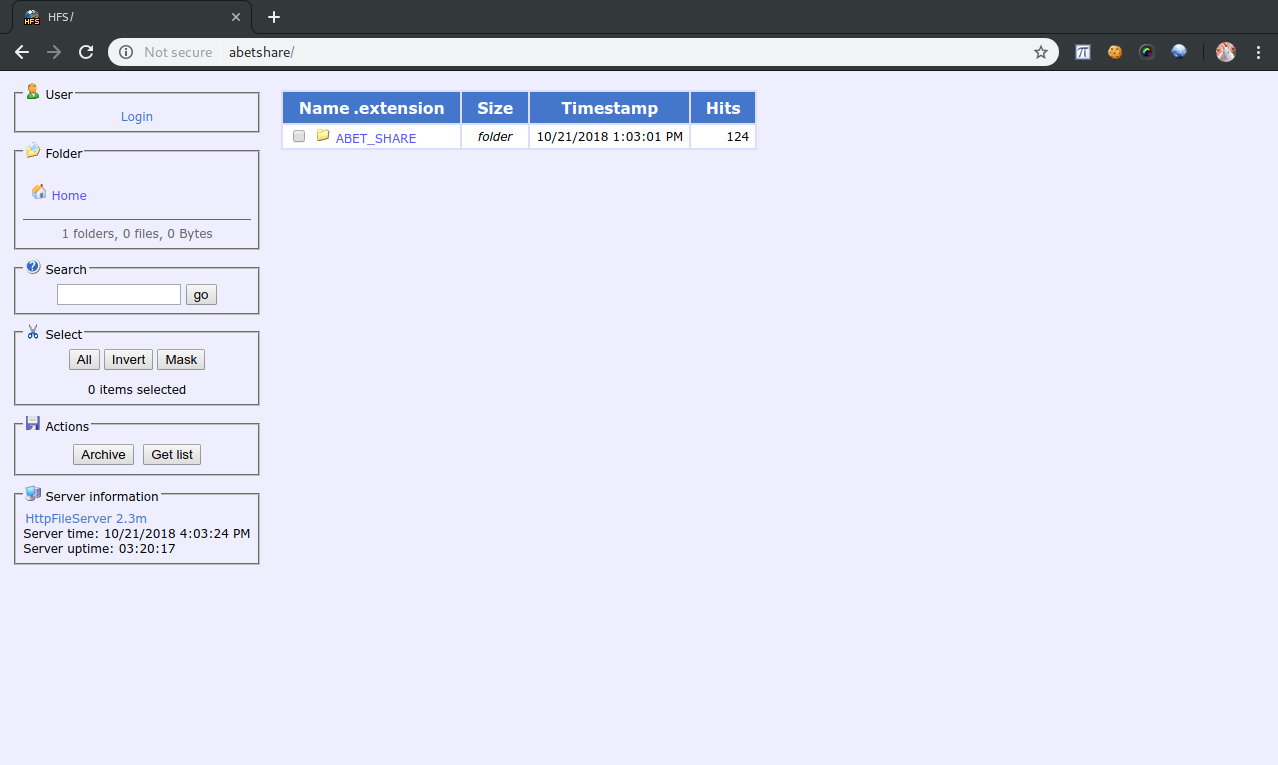
\includegraphics[scale=0.30]{./img/fileshare/01_htf_home.png}
  \caption{Fileshare Client}
  \label{fig:01_htf_home}
\end{figure}

\begin{figure}[H]
  \centering
  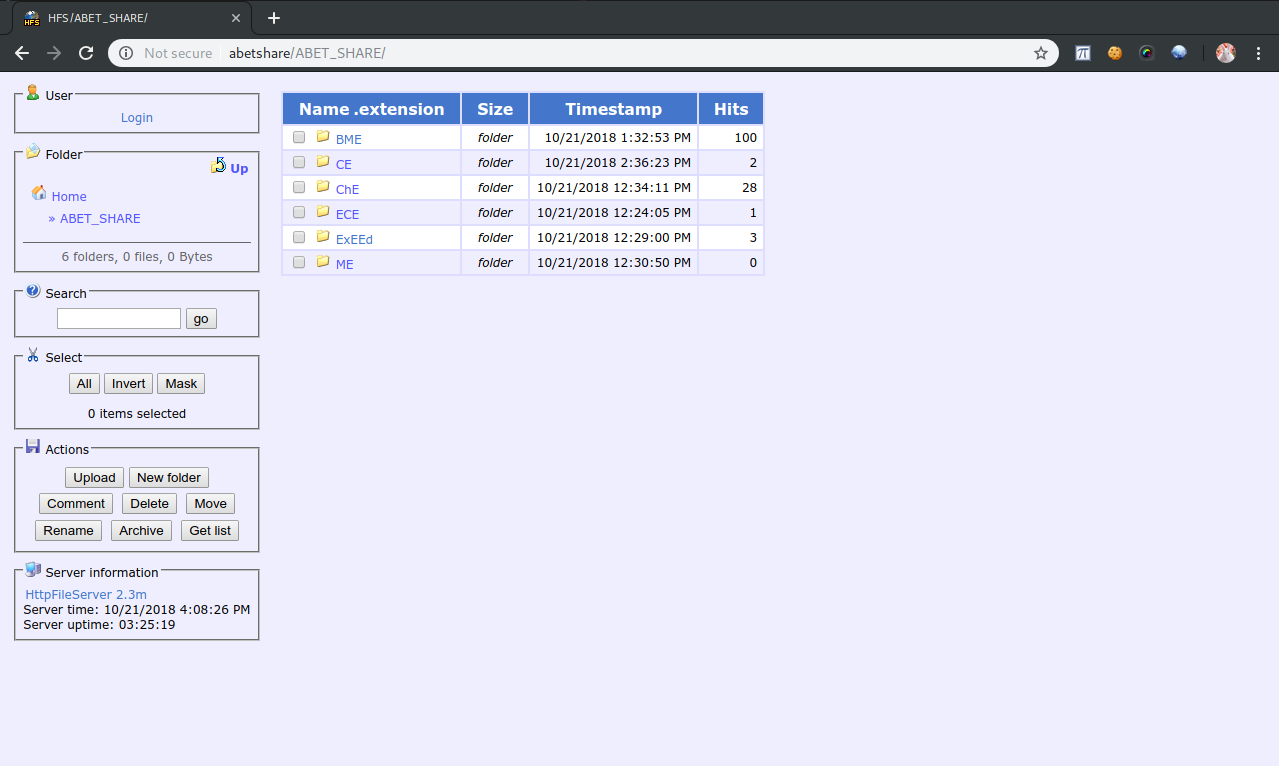
\includegraphics[scale=0.30]{./img/fileshare/02_hfs_abet_share.png}
  \caption{HFS Client}
  \label{fig:02_hfs_abet_share}
\end{figure}



%
%\subsubsection{Fileshare Description}
%\textbf{The following are the set of instructions given to ABET users for
%  accessing the fileshare}
%In order to make sharing documents as seamless as possible, a local fileshare
%server is setup on the ABET network where all users on the network can access
%and upload documents to a shared folder. Users can upload/download documents
%to/from the fileshare folder from any device via any web browser (no additional
%software is needed).
%\\\\
%To access the fileshare:
%\begin{enumerate}
%  \item{Connect your device to ABET\_WiFi}
%%   \\
%%   This can be done via connecting the device to ABET\_WiFi or using either of
%%   the desktop workstations in the Dean's conference room.
%
%  \item{Go to \url{http://abetshare/}}
%    \\
%    On your network-connected device, open a web browser and type
%    \url{http://abetshare/} in the address bar and press [ENTER]. This should
%    direct you to the fileshare webpage.
%
%  \item{Using the fileshare}
%    \\
%    The fileshare webpage will display an ABET\_SHARE folder, this is where the
%    fileshare documents are contained. Click the ABET\_SHARE folder to open it.
%    The fileshare webpage behaves similarly to a desktop file explorer, you can
%    navigate through folders and open files by clicking them. The menu on the
%    left side of the webpage has additional options such as upload, delete, and
%    create new folder.
%
%\end{enumerate}
%
%\subsection{Using the Desktop Workstations}
%
%There are two, complimentary Windows workstations located in the Dean's
%conference room that are connected to the ABET network. \textbf{No credentials are
%required to sign in}.
%\\\\
%There is a special \textbf{Desktop\textbackslash ABET\_SHARE} folder on each
%workstation that is automatically synced to the ABET fileshare. This means
%that both workstations will automatically update the contents of
%this folder with the documents in the network fileshare so you can simply treat the
%fileshare like a regular system folder. Adding files to the ABET\_SHARE
%folder uploads them to the fileshare, files uploaded to the fileshare are
%automatically downloaded and appear in the ABET\_SHARE folder.

\end{document}
